
\chapter{Software Design}

\section{Einführung}

\section{,,Das Problem''}

Da die grundlegende Funktionsweise des MPD Server auf einer Client Server Architektur beruht, muss der MPD Client
verschiedene Kommandos wie zum Beispiel \it play, pause, listplaylists \rm etc. an den Server schicken können
und zur gleichen Zeit aber auch auf Änderungen reagieren können, d.h. zum Beispiel wenn sich die Lautstärke ändert,
da jederzeit auch andere Clients oder Server den MPD internen Zustand ändern können.
Diese Änderungen müssen auch anderen Programmteilen bekannt gemacht werden.
Für die Realisierung eignet sich hier das Observer Pattern gut. \footnote{http://de.wikipedia.org/wiki/Observer\_(Entwurfsmuster)}
\\
Der Client sollte im ,,idle''-Mode möglichst keine Ressourcen verschwenden und auch beim 
trennen und verbinden die entsprechenden Änderungen anderen Teilen des Programms mitteilen
können. 
\\

Das MPD Protokoll \footnote{http://www.musicpd.org/doc/protocol/index.html} bietet folgende Möglichkeiten das zu realisieren
\begin{description}
    \item [Periodisch] (zB. alle 500ms) das ,,\textit{status}'' Kommando absetzen und nach Bedarf auch Kommandos wie ,,\textit{currentsong}''
        senden.
        \\
        \emph{Problem:} Bei langsamen Netzwerkverbindungen erzeugt dies unnötige Netzwerklast. 
        Prinzipiell würde sich auf diese Art jedoch z.B. die Musik Bitrate anzeigen lassen. Es ist jedoch ein
        wenig komfortabler Weg da hier wieder einmal das Rad neu erfunden werden müsste, denn man müsste manuell raus finden 
        was genau sich eigentlich geändert hat.
    \item [Nutzung der ,,\textit{idle}'' und ,,\textit{noidle}'' commands:]
        ,,\textit{idle}'' versetzt die Verbindung zum Server in einen Schlafzustand. Sobald Events wie ,,\textit{player}'' (wird beispielsweise durch pausieren getriggert) 
        eintreten, wacht die Verbindung aus diesem Zustand auf und sendet an den Client eine Liste der Events die aufgetreten sind:

	\begin{figure}[h!]
	  \lstinputlisting[language=bash]{./src/state.txt}
	  \caption{Eine Beispielantwort des MPD Servers}
	  \label{dd_state}
	\end{figure}

        Allerdings gibt es hier eine weitere Einschränkung: Während die Verbindung im idle mode ist kann kein reguläres Kommando wie ,,\textit{play}'' gesendet werden!
        Sollte man es doch tun wird man augenblicklich vom Server getrennt.
        Die einzige Möglichkeit aus dem idle mode aufzuwachen ist das ,,\textit{noidle}'' Kommando, das gesendet werden
        kann während die Verbindung schlafen gelegt wurde.
        Jedoch gibt es auch hier ein Problem, denn das ,,\textit{idle}'' Kommando blockiert, sprich es sendet kein ,,OK'' an den  Sender zurück.
        Ein Warten auf dieses ,,OK'' würde mit den Wunsch eine in der Zwischenzeit bedienbare Oberfläche zu haben kollidieren.
\end{description}

Prinzipiell gibt es 2 Möglichkeiten dieses Problem zu lösen:
\begin{itemize}
    \item Man hält zwei Verbindungen zum Server, eine die Kommandos sendet, eine die stets im ,,\textit{idle}'' mode liegt,
        Für die Realisierung müssten Threads herangezogen werden. Ein Thread würde dann im Hintergrund auf Events lauschen,
        der andere würde zum Abschicken der Kommandos benutzt werden.
        \emph{Problem:} Es müssen 2 Verbindungen gehandelt werden, was wiederum ein Mehraufwand an Code bedeutet.
        Desweiteren werden Threads benötigt die auch in anderen Bereichen des Programms Lockingmechanismen bedeuten würden.
    \item Man hält eine asynchrone Verbindung zu dem Server.
        Diese kann das ,,\textit{idle}'' Kommando zum Server schicken, gibt aber sofort die Kontrolle dem Aufrufer zurück. Um nun eine Liste der events zu bekommen setzt man 
        einen ,,\textit{Watchdog}''auf die asynchrone Verbindung an (Vergleiche dazu den Systemaufruf ,,man 3 poll'').
        Da poll() ebenfalls den aufrufenden Prozess blockiert, wird die Glibfunktion\footnote{GLib ist eine Utility Bibliothek für C die von Gtk+ genutzt wird} Glib::signal\_io() benutzt, das sich in den laufenden MainLoop\footnote{Siehe MainLoop im Glossar} einhängt und eine 
        Callbackfunktion aufruft sobald auf der Verbindung etwas Interessantes passiert. Da während des Wartens der MainLoop
        weiterarbeitet, bleibt die GUI (und andere Module) aktiv und benutzbar.
        \\
        \emph{Problem:} Vor dem Senden eines Kommandos wie ,,\textit{play}'' muss der idle mode verlassen werden.
        \emph{Lösung:} Man kann das ,,\textit{noidle}'' Kommando zum Verlassen senden, und nach dem Absenden des eigentlichen Kommandos wieder den idle-mode betreten.
\end{itemize}

Zum Verständnis der Problematik wird hier eine telnetsession gezeigt. 
Über telnet kann man das MPD Protokoll ,,interaktiv'' benutzen und ausprobieren: 
% Insert telnet session
\lstinputlisting[language=bash]{./src/telnet.txt}

Die Idee zu dieser Implementierung (speziell das Benutzen einer asynchronen Verbindung), kommt von ,,\textit{ncmpc}'',
der mehr oder minder offiziellen Referenzimplementierung des MPD Mit-Authors \emph{Max Kellermann}.
Vergleiche \href{http://mpd.wikia.com/wiki/Client:Ncmpc}{ncmpc quellcode}: \textit{src/gidle.c} und \textit{src/mpdclient.c}
\begin{figure}[htb!]
\subsection{Aufbau der Anwendung}
	\centering
        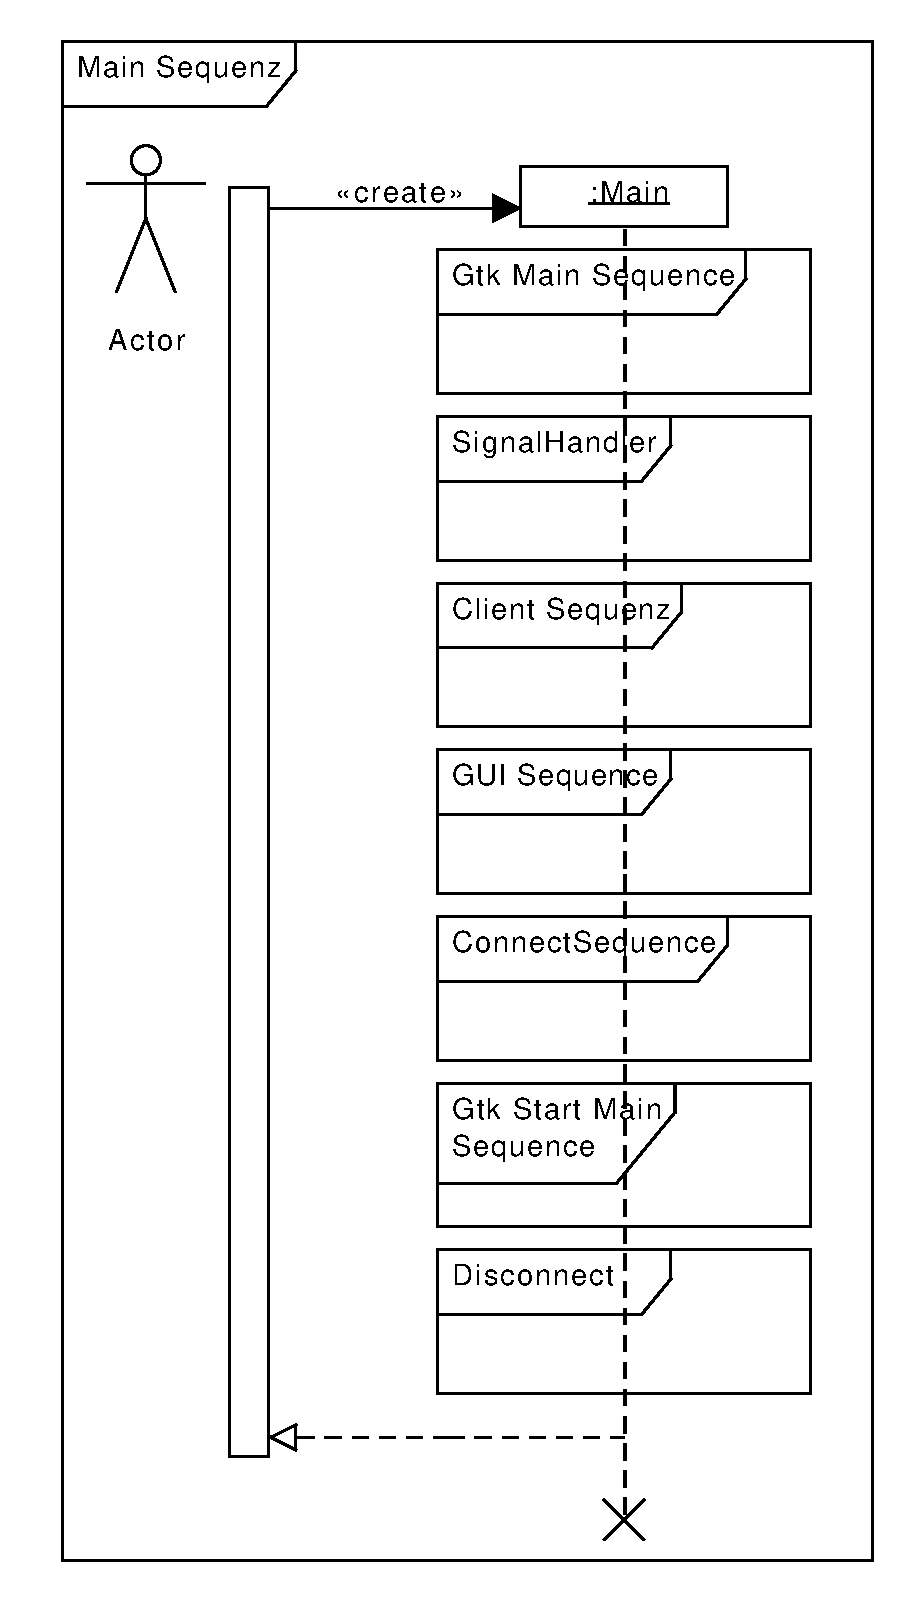
\includegraphics[scale=0.3]{./gfx/seq/main}
	\caption{Die Initialisierungsphase}
	\label{seq_main_init}
\end{figure}

% Reihenfolge in der aufgebaut wird 
\newpage

